\section{Пример: коэффициент корреляции}

Мы уже видели два примера бутстреп оценок стандартной ошибки для среднего и медианного значения для экспериментальной группы данных о мышах, таблица 2.1. В качестве второго примера рассмотрим выборочный коэффициент корреляции между $y = LSAT$ и $z = GPA$ для $n = 15$ точек данных о юридических школах, таблица 3.1, $\widehat{corr}(y, z) =0.776$. Насколько точна оценка $0.776$? В таблице 6.1 показана бутстреп оценка стандартной ошибки $\widehat{se}_B$ для $B$ в диапазоне от $25$ до $3200$. Последнее значение, $\widehat{se}_{3200} = 0.132$, является нашей оценкой $se_F (\widehat{corr})$. Позже мы увидим, что $\widehat{se}_{200}$ почти так же хороша для оценки $se_F$, как $\widehat{se}_{3200}$· 

Глядя на правую часть рисунка 3.1, читатель может представить себе, как работает генерация бутстреп выборок. Выборочная корреляция по $n = 15$ исходным точкам данных составляет $\widehat{corr} = 0.776$. Бутстреп выборка состоит из $15$ точек, выбранных случайным образом и заменяющих исходные $15$. Корреляция бутстреп выборки представляет собой бутстреп репликацию $\widehat{corr}^*$, которая может быть больше или меньше, чем $\widehat{corr}$. Независимые повторения генерации бутстреп выборок дают бутстреп репликации $\widehat{corr}^*(1),\widehat{corr}^*(2),\cdots,\widehat{corr}^*(B)$. Наконец, $\widehat{se}_B$ -- выборочное стандартное отклонение значений $\widehat{corr}^*(b)$. 
\newline

\noindent
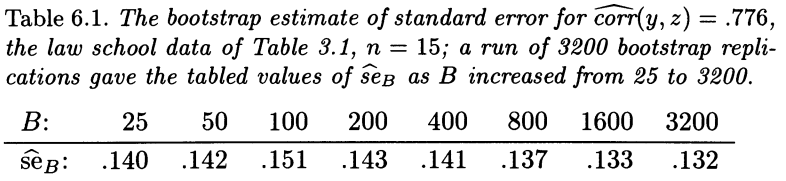
\includegraphics[width=\linewidth]{5/t61.png}
\newline

Левая панель рисунка 6.2 представляет собой гистограмму $3200$ бутстреп репликаций $\widehat{corr}^*(b)$. Всегда рекомендуется просматривать бутстреп данные графически, а не полагаться полностью на одну сводную статистику, такую как $\widehat{se}_B$. В примере корреляции может оказаться, что несколько выпадающих значений $\widehat{corr}^*(b)$ сильно раздувают $\widehat{se}_B$, и в этом случае стоит использовать более надежную меру стандартного отклонения; Выводы, основанные на нормальной кривой, как в (5.6) и на рисунке 5.1, сомнительны, когда бутстреп гистограмма явно ненормальна.

В примере с юридическими школами у нас есть полная совокупность $\mathbf{X}$ из $N = 82$ школ, Таблица 3.2. В правой части рисунка 6.2 показана гистограмма $\widehat{corr} (y, z)$ для $3200$ выборок размера $n = 15$, взятых из $\mathbf{X}$. Другими словами, $3200$ случайных выборок $\mathbf{x} = (x_1, x_2, \cdots, x_{15})$ были составлены с заменой из $82$ точек в $\mathbf{X}$, и $\widehat{corr}(\mathbf{x})$ оценивался для каждого из них. Стандартное отклонение $3200$ значений $\widehat{corr}(\mathbf{x})$ составило $0.131$, таким образом $\widehat{se}_B$ является хорошей оценкой стандартной ошибки генеральной совокупности. Что еще более впечатляюще, бутстреп гистограмма слева сильно напоминает гистограмму справа. Помните, что в реальной проблеме у нас была бы только информация слева, из которой мы пытались бы вывести ситуацию справа. 
\newline

\noindent
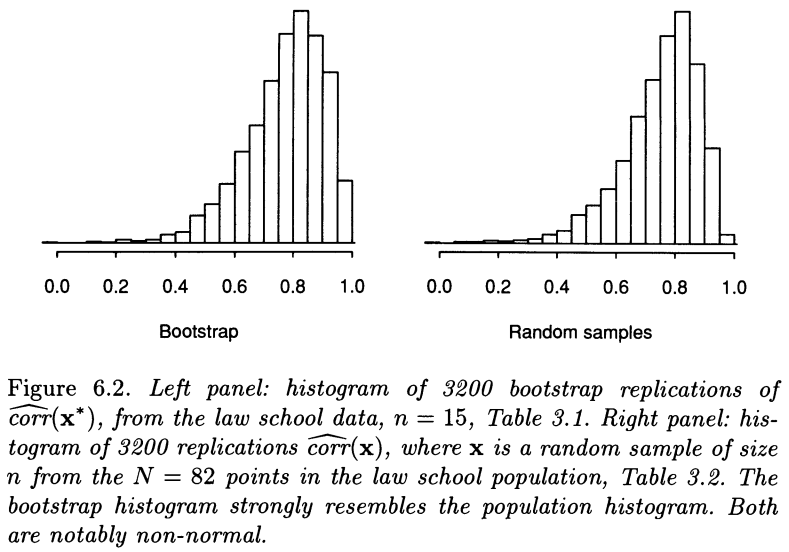
\includegraphics[width=\linewidth]{5/f62.png}
\newline